\documentclass[12pt]{report}
\usepackage[a4paper,margin=1in]{geometry}
\usepackage{setspace}
\usepackage{graphicx}
\usepackage{sectsty}
\usepackage{pdfpages}
% \usepackage{booktabs}
\usepackage[export]{adjustbox}
\usepackage{amssymb}
\usepackage{cancel}
\usepackage[numbered]{matlab-prettifier}
\usepackage{circuitikz}
\usepackage{xfrac}
\usepackage{lmodern}
\usepackage{multicol}
\usepackage{caption}
\usepackage{amsmath}

\usetikzlibrary{arrows}
\graphicspath{{images/}}
\usetikzlibrary{calc,patterns,angles,quotes}

\allsectionsfont{\centering}
\renewcommand\thesection{\arabic{section}}
\renewcommand{\thefootnote}{\arabic{footnote}}
\setcounter{tocdepth}{5}

\begin{document}

\input{titlepage}
\pagenumbering{roman}
{\tableofcontents\let\clearpage\relax\listoffigures}
\clearpage
\pagenumbering{arabic}
\newpage
\begin{flushleft}
% ---------------------------------------------------------------------------- %
\section{Conceptualize the Problem}
% ---------------------------------------------------------------------------- %

The first step to solving the problem is to conceptualize the system and understand what is being asked for. The idealized pendulum is a 1 degree of freedom (DOF) problem, and the best coordinate system to model the system is either normal-tangential ($\hat{e}_n,\hat{e}_t$) or polar ($\hat{e}_r,\hat{e}_\theta$); this way the position of the mass is easily shown using only one variable, $\theta$, and since most of the forces act tangentially on the mass, calculations made later will be less strenuous. We will be using a normal-tangential coordinate system.

\subsection{Constants and Assumptions}

\begin{figure}[h]
  \centering
   \begin{minipage}[c]{.2\textwidth}
      \usetikzlibrary{calc,patterns,angles,quotes}
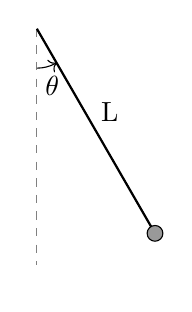
\begin{tikzpicture}
    % save length of g-vector and theta to macros
    \pgfmathsetmacro{\Gvec}{1.5}
    \pgfmathsetmacro{\myAngle}{30}
    % calculate lengths of vector components
    \pgfmathsetmacro{\Gcos}{\Gvec*cos(\myAngle)}
    \pgfmathsetmacro{\Gsin}{\Gvec*sin(\myAngle)}

    \coordinate (centro) at (0,0);
    \draw[dashed,gray,-] (centro) -- ++ (0,-3) node (mary) [black,below]{$ $};
    \draw[thick] (centro) -- ++(270+\myAngle:3) coordinate (bob);
    \pic [draw, ->, "$\theta$", angle eccentricity=1.5] {angle = mary--centro--bob};
    \draw (bob) -- (centro) node[midway, above]{~~~L};
    \filldraw [fill=black!40,draw=black] (bob) circle[radius=0.1];
\end{tikzpicture}

   \end{minipage}%
   \begin{minipage}[c]{.8\textwidth}
     \begin{tabular}{ll@{\hskip .75in}l}
       \multicolumn{1}{c}{Constants:} && \multicolumn{1}{c}{Assumptions:} \\
       Mass: &m = 0.142kg & Frictionless\\
       String Length: &L = 0.5m & Released from Rest\\
       Gravity: &g = 9.81$\sfrac{m}{s^2}$ & Particle Dynamics\\
     \end{tabular}
   \end{minipage}
 \end{figure}

The system is released from rest at various initial angles of release:
$$\theta_o = 5^\circ,10^\circ, 15^\circ, 30^\circ, 60^\circ, \textrm{and}~90^\circ$$
Drag force is defined as
\begin{equation} \label{eq:drag}
\bar{F}_{Drag}=\frac{1}{2}\rho C_DAV^2\left(-\hat{V}\right)=-1.65 \cdot10^{-3}\dot{\theta}|\dot{\theta}|\hat{e_t}
\end{equation}
We are also asked to determine the following: \\
\begin{equation}
\textrm{With and Without Drag\quad}\left\{
\begin{array}{ll}
  \textrm{Equations of Motion}& \\
  \textrm{Natural Frequency } &\hspace{10ex}\omega_n\hspace{1.5ex} \\
\end{array}
\nonumber
\right.
\end{equation}
\begin{equation}
\textrm{\phantom{and Without}With Drag\quad}\left\{
\begin{array}{ll}
  \textrm{$2^{nd}$ Order Diff. Eq. of Motion} & \\
  \textrm{Damped Natural Frequency } &\omega_d \\
  \textrm{The Damping Ratio} & \zeta \\
  \textrm{The Decay Rate} & \zeta\omega_n \\
\end{array}
\right.
\nonumber
\end{equation}
\newpage

% ---------------------------------------------------------------------------- %
\section{Free Body Diagram}
% ---------------------------------------------------------------------------- %

\begin{figure}[ht]
  \centering
   \begin{minipage}[c]{.2\textwidth}
      
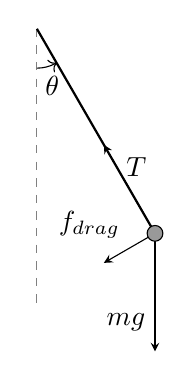
\begin{tikzpicture}
    % save length of g-vector and theta to macros
    \pgfmathsetmacro{\Gvec}{1.5}
    \pgfmathsetmacro{\myAngle}{30}
    % calculate lengths of vector components
    \pgfmathsetmacro{\Gcos}{\Gvec*cos(\myAngle)}
    \pgfmathsetmacro{\Gsin}{\Gvec*sin(\myAngle)}

    \coordinate (centro) at (0,0);
    \draw[dashed,gray,-] (centro) -- ++ (0,-3.5) node (mary) [black,below]{$ $};
    \draw[thick] (centro) -- ++(270+\myAngle:3) coordinate (bob);
    \pic [draw, ->, "$\theta$", angle eccentricity=1.5] {angle = mary--centro--bob};
    \draw [black,-stealth] (bob) -- ($(bob)!\Gcos cm!(centro)$)
      coordinate (T)
      node[near end, right] {$T$};
    \draw [-stealth] (bob) -- ($(bob)!\Gsin cm!90:(centro)$)
      coordinate (gsin)
      node[midway,above left] {$f_{drag}$};
    \draw [-stealth] (bob) -- ++(0,-\Gvec)
      coordinate (g)
      node[near end,left] {$mg$};
    % \pic [draw, ->, "$\theta$", angle eccentricity=1.5] {angle = g--bob--gcos};
    \filldraw [fill=black!40,draw=black] (bob) circle[radius=0.1];
\end{tikzpicture}

   \end{minipage}%
   \begin{minipage}[c]{.8\textwidth}
     \flushleft
     \begin{tabular}{rl}
     $f_{Drag}$:&Drag force$^*$ acting against the velocity of the mass (-$\hat{v}$)\\
     $mg$:&Mass $\cdot$ gravity, the weight of the object\\
     $T$:&The tension in the string\\
   \end{tabular}
     \footnotetext{$^*$Modeled by Eq.(\ref{eq:drag})}
   \end{minipage}
 \end{figure}

% ---------------------------------------------------------------------------- %
\section{Coordinate Frame}
% ---------------------------------------------------------------------------- %

\begin{figure}[h]
  \centering
   \begin{minipage}[c]{.15\textwidth}
      \begin{tikzpicture}
    % save length of g-vector and theta to macros
    \pgfmathsetmacro{\Gvec}{1.5}
    \pgfmathsetmacro{\myAngle}{30}
    % calculate lengths of vector components
    \pgfmathsetmacro{\Gcos}{\Gvec*cos(\myAngle)}
    \pgfmathsetmacro{\Gsin}{\Gvec*sin(\myAngle)}

    \coordinate (centro) at (0,0);
    \coordinate (bob) at (270+\myAngle:3);
    \draw [black,-stealth] (bob) -- ($(bob)!\Gcos cm!(centro)$)
      coordinate (T)
      node[above] {$\hat{e_n}$};
    \draw [-stealth] (bob) -- ($(bob)!\Gsin cm!-90:(centro)$)
      coordinate (gsin)
      node[above] {$\hat{e_t}$};
      \phantom{
        \draw [-stealth] (bob) -- ++(0,-\Gvec)
          coordinate (g)
          node[near end,left] {$mg$};
        }
    \filldraw [fill=black!40,draw=black] (bob) circle[radius=0.1];
\end{tikzpicture}

   \end{minipage}%
   \begin{minipage}[c]{.85\textwidth}
     \flushleft
     \begin{tabular}{rl}
      $\hat{e}_n$:&+ Pointing at the centroidal point about which the system rotates\\
      $\hat{e}_t$:&+ Pointing in the direction that represents counterclockwise \\
      & \phantom{+ }tangential movement about the centroidal point \\
    \end{tabular}
   \end{minipage}
 \end{figure}
We determined the positive direction for the coordinate system based on planar dynamics
conventions.
% ---------------------------------------------------------------------------- %
\section{Sum of Forces}
% ---------------------------------------------------------------------------- %

$$\sum\bar{F}=m\bar{a}_{cm}$$
Since we are using a normal-tangential coordinate system,
$$
\bar{a}_{cm} =
\begin{bmatrix}
r\dot{\theta}^2\\
r\ddot{\theta}
\end{bmatrix}
$$
There are no moments in this problem that are accounted for. \\
~\\
Without drag:
\center{Sum of the forces in the normal direction,}
\begin{equation} \label{eq:fn}
\sum F_n = -mg\cos(\theta) + m(L\dot{\theta}^2) = 0
\end{equation}
\center{Sum of the forces in the tangential direction.}
\begin{equation} \label{eq:ft}
\sum F_t = m(L\ddot{\theta}) - mg\sin(\theta) = 0
\end{equation}
\newpage
\flushleft {With drag:\\}
\center{Sum of the forces in the normal direction,}
\begin{equation} \label{}
\sum F_n = -mg\cos(\theta) + m(L\dot{\theta}^2) = 0
\end{equation}
\center{Sum of the forces in the tangential direction.}
\begin{equation}
\sum F_t = m(L\ddot{\theta}) - mg\sin(\theta) - F_{Drag} = 0
\end{equation}
\flushleft
Where: \\
~\\
\begin{tabular}{rl}
$F_n$:& Denotes the forces acting in the normal direction. \\
$F_t$:& Denotes the forces acting in the tangential direction. \\
$\theta$:& Position of the mass. \\
$\dot{\theta}$:& Angular velocity of the mass. \\
$\ddot{\theta}$:& Angular acceleration of the mass. \\
m, L, g: & Are constants; mass, length of string, and gravity, respectively
\end{tabular}
% ---------------------------------------------------------------------------- %
\section{Knowns and Unknowns} \label{knownsandunknowns}
% ---------------------------------------------------------------------------- %
\begin{tabular}{ll@{\hskip .75in}ll}
  \multicolumn{1}{c}{Knowns:} && \multicolumn{1}{c}{Unknowns:} \\
  % Knowns: && Unknowns: &\\
  Mass: &m = 0.142kg & String Tension: & T \\
  String Length: &L = 0.5m & Angular Acceleration: & $\ddot{\theta}$ \\
  Gravity: &g = 9.81$\sfrac{m}{s^2}$ \\
  State Variables: \\
  \quad Angular Velocity: &$\dot{\theta}$ & \\
  \quad Angular Acceleration:&$\ddot{\theta}$ & \\
\end{tabular}
\vspace{2ex}
\\
The angular velocity and position state variables are associated with the angular
acceleration, so they are considered known since they can be obtained from the
acceleration using integration. Therefore we have two equations of motion
(\ref{eq:fn}) \& (\ref{eq:ft}) and two unknowns (T and $\ddot{\theta}$).
% ---------------------------------------------------------------------------- %
\section{Constraints}
% ---------------------------------------------------------------------------- %
Since there are as many unknowns as there are equations, constraints are not needed
in this problem. \\
% ---------------------------------------------------------------------------- %
\section{Solve for the Equations of Motion}
% ---------------------------------------------------------------------------- %
The equations of motion for a simple pendulum are
 (from Eq. (\ref{eq:fn}) and (\ref{eq:ft}))
\begin{equation} \label{eq:pen}
\ddot{\theta} = -\frac{g}{L}\sin(\theta)
\end{equation}
\center and
\begin{equation} \label{eq:T}
T = mg\cos(\theta) + mL\dot{\theta}^2
\end{equation}
Whereas with drag, the only difference is in Eq. (\ref{eq:pen}); plugging in
the drag force representation (from Eq. (\ref{eq:drag}))
\begin{equation}\label{eq:drageom}
  \ddot{\theta} = -\frac{g}{L}\sin(\theta) - \frac{1.65 \cdot 10^{-3}\dot{\theta}|\dot{\theta}|}{mL}
\end{equation}
% ---------------------------------------------------------------------------- %
\section{Solve the Equations of Motion}
% ---------------------------------------------------------------------------- %
\subsection{Without Drag}
\flushleft
Taking Equation (\ref{eq:pen}),
$$\ddot{\theta} = -\frac{g}{L}\sin(\theta)$$
We can integrate the differential equation using MATLAB and plot the behavior of
$\theta$ versus time for various release angles. (Figure (\ref{fig:thetatime})) \\
\begin{figure}[h]
\begin{minipage}[c]{.85\textwidth}
  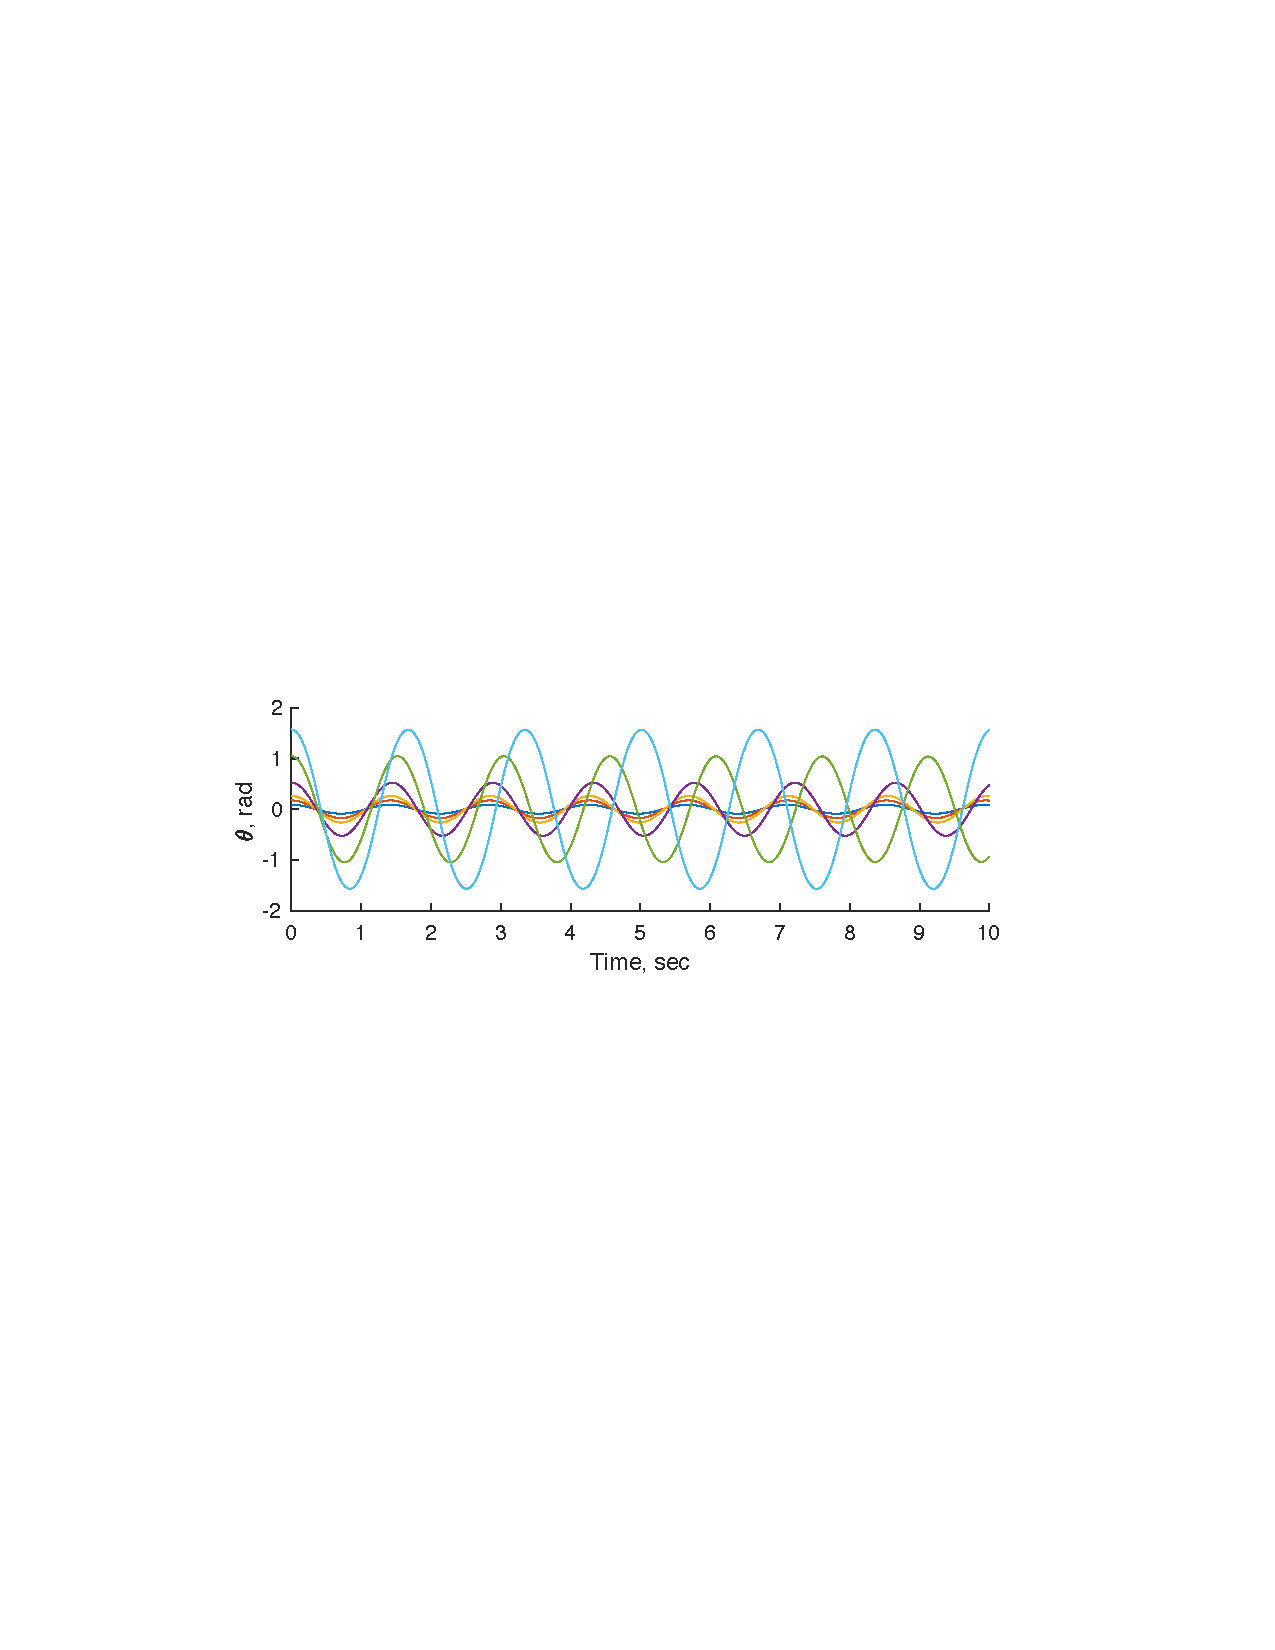
\includegraphics[center,width=.9\textwidth]{theta}
\end{minipage}%
\begin{minipage}[c]{.15\textwidth}
  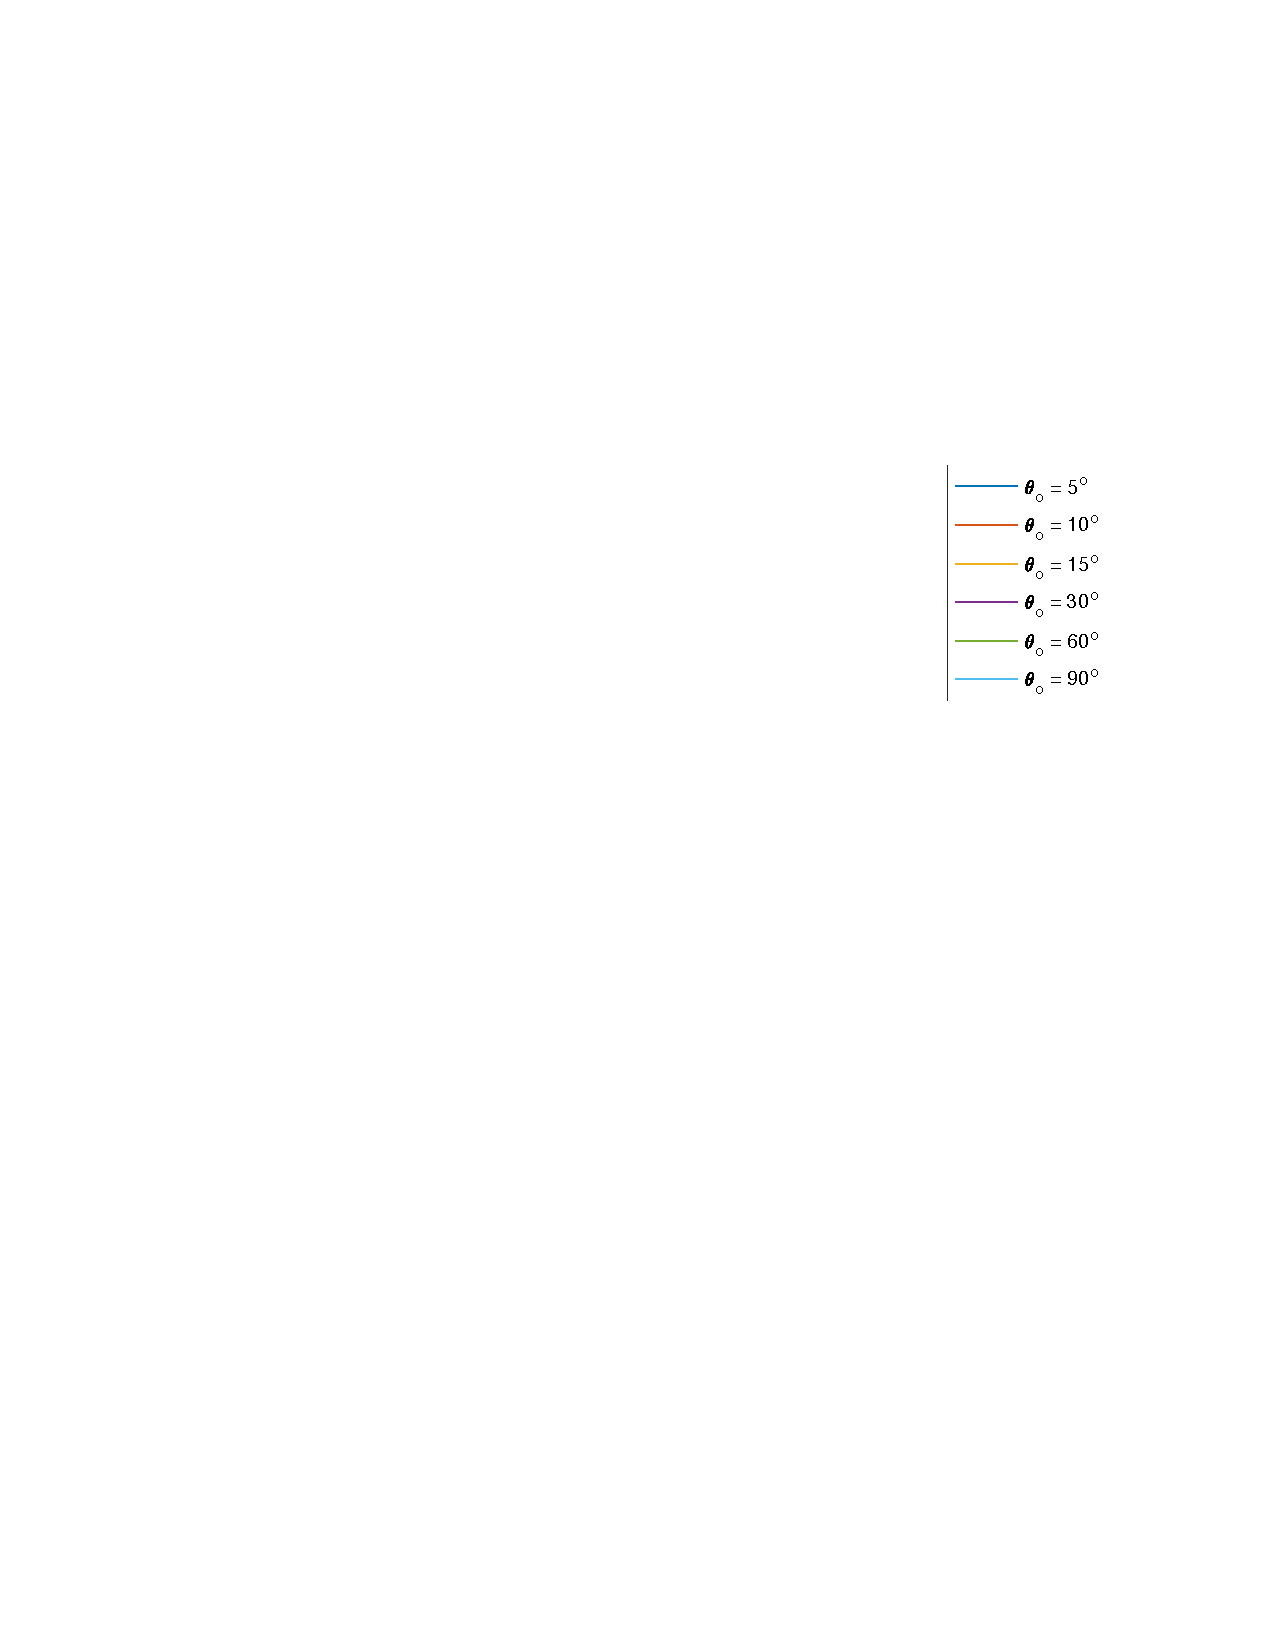
\includegraphics[frame,center]{thetalegend}
  \vspace{1ex}
\end{minipage}
  \caption{$\theta$ vs Time For Various Initial Release Angles}
  \label{fig:thetatime}
\end{figure}
~\\
Using the small angle approximation ($\sin(\theta)\approx\theta$), we can rewrite
Equation (\ref{eq:pen}) as
$$\ddot{\theta} = -\frac{g}{L}\theta$$
Letting $\theta(t) = A\cdot e^{st}$, then $\ddot{\theta} = s^2 \cdot A \cdot e^{st}$;
solving the second order differential equation analytically yields
$$\theta(t) = \theta_o\cos(\sqrt{\frac{g}{L}t})$$
Where
$$\sqrt{\frac{g}{L}} = \omega_n$$
\begin{figure}[ht]
  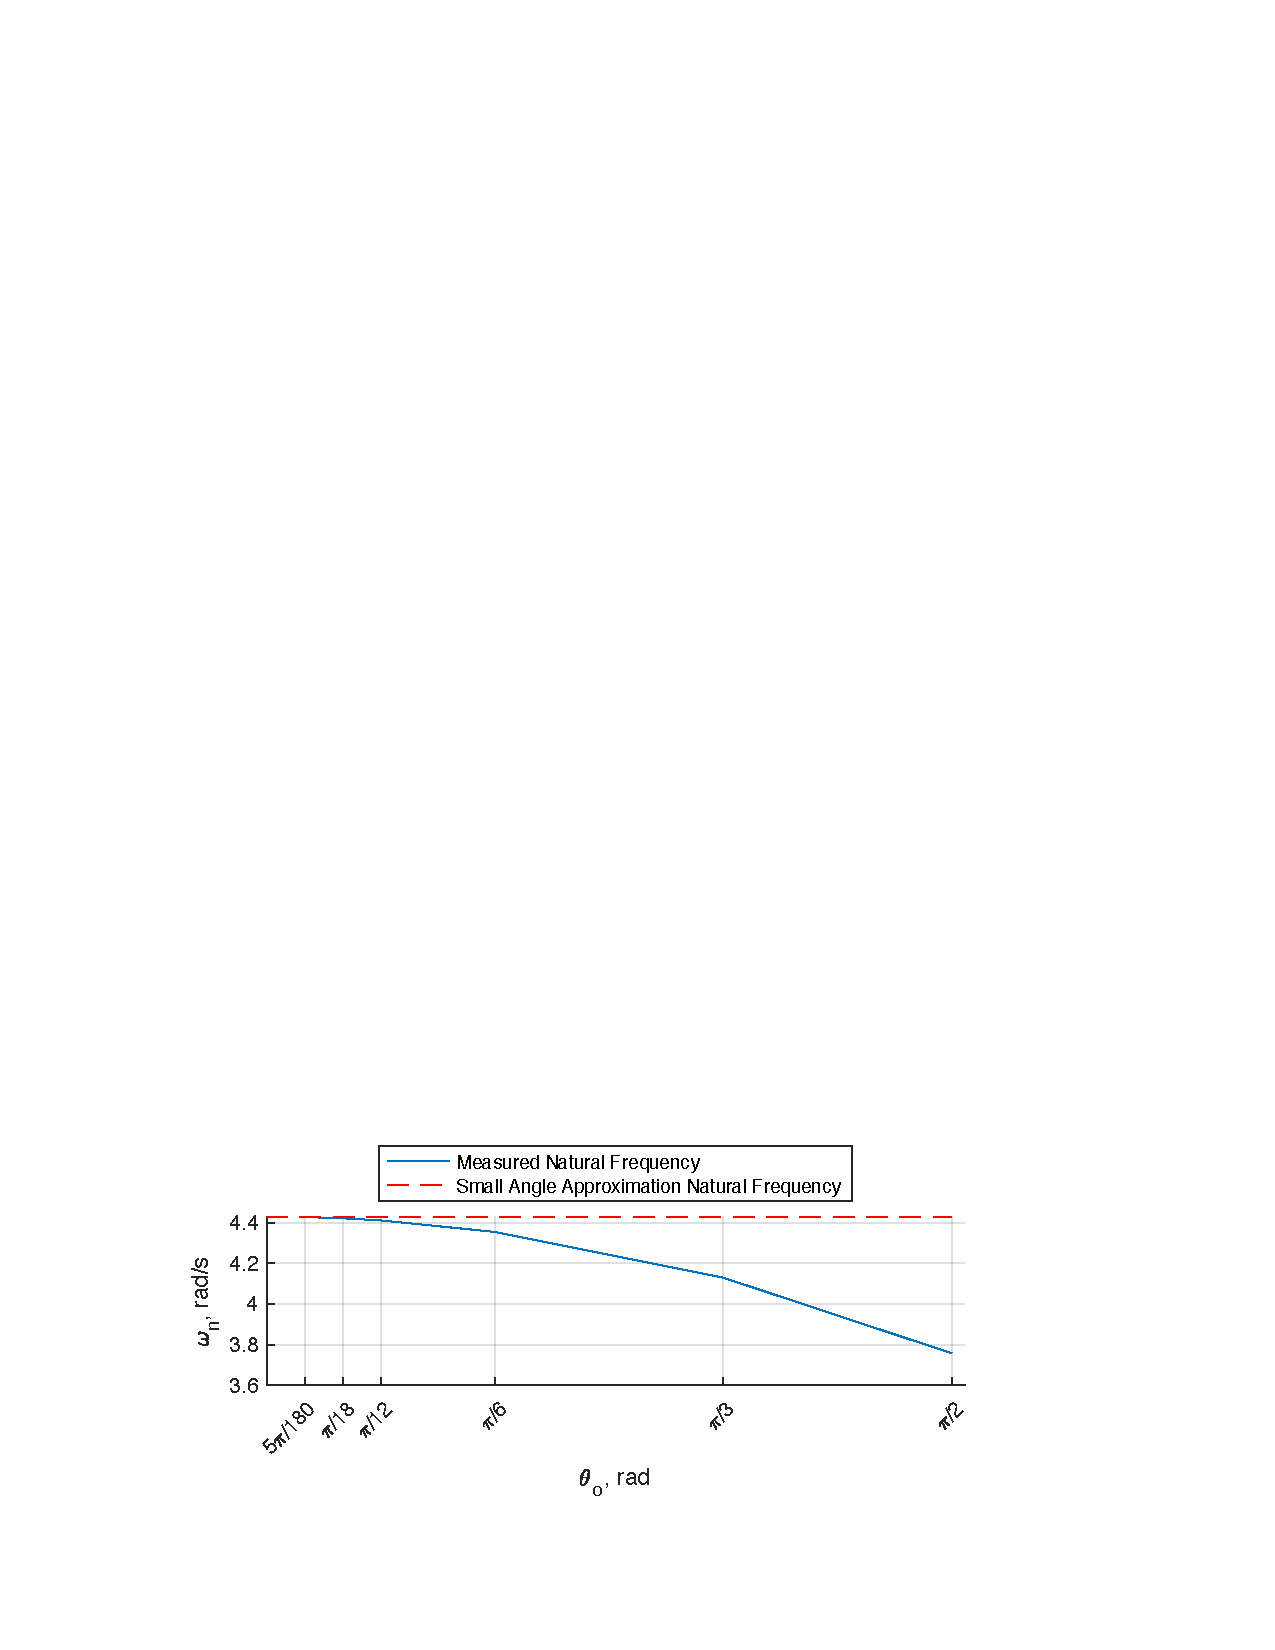
\includegraphics[center,width=.9\textwidth]{natfreq}
  \caption{Natural Frequency ($\omega_n$) vs Initial Angle of Release ($\theta_o$)}
  \label{fig:freq}
\end{figure}
\newpage
As shown in Figure (\ref{fig:freq}), using the small angle approximation has very
little effect on the calculation of the natural frequency of the system, especially
when $\theta_o$ is smaller in magnitude; later on when the small angle
approximation is used to represent the system with drag incorporated, the initial
angle of release, $\theta_o$, is $\sfrac{\pi}{12}$. As seen in Figure (\ref{fig:freq}),
the value of $\omega_n$ at $\sfrac{\pi}{12}$ using the approximation is very
close to the actual frequency of the system.

\subsection{With Drag}
Using Equation (\ref{eq:drageom})
$$
\ddot{\theta} = -\frac{g}{L}\sin(\theta) - \frac{1.65 \cdot 10^{-3}\dot{\theta}|\dot{\theta}|}{mL}
$$
We can integrate and plot the differential equation over a 100 second period. \\
\begin{figure}[ht]
  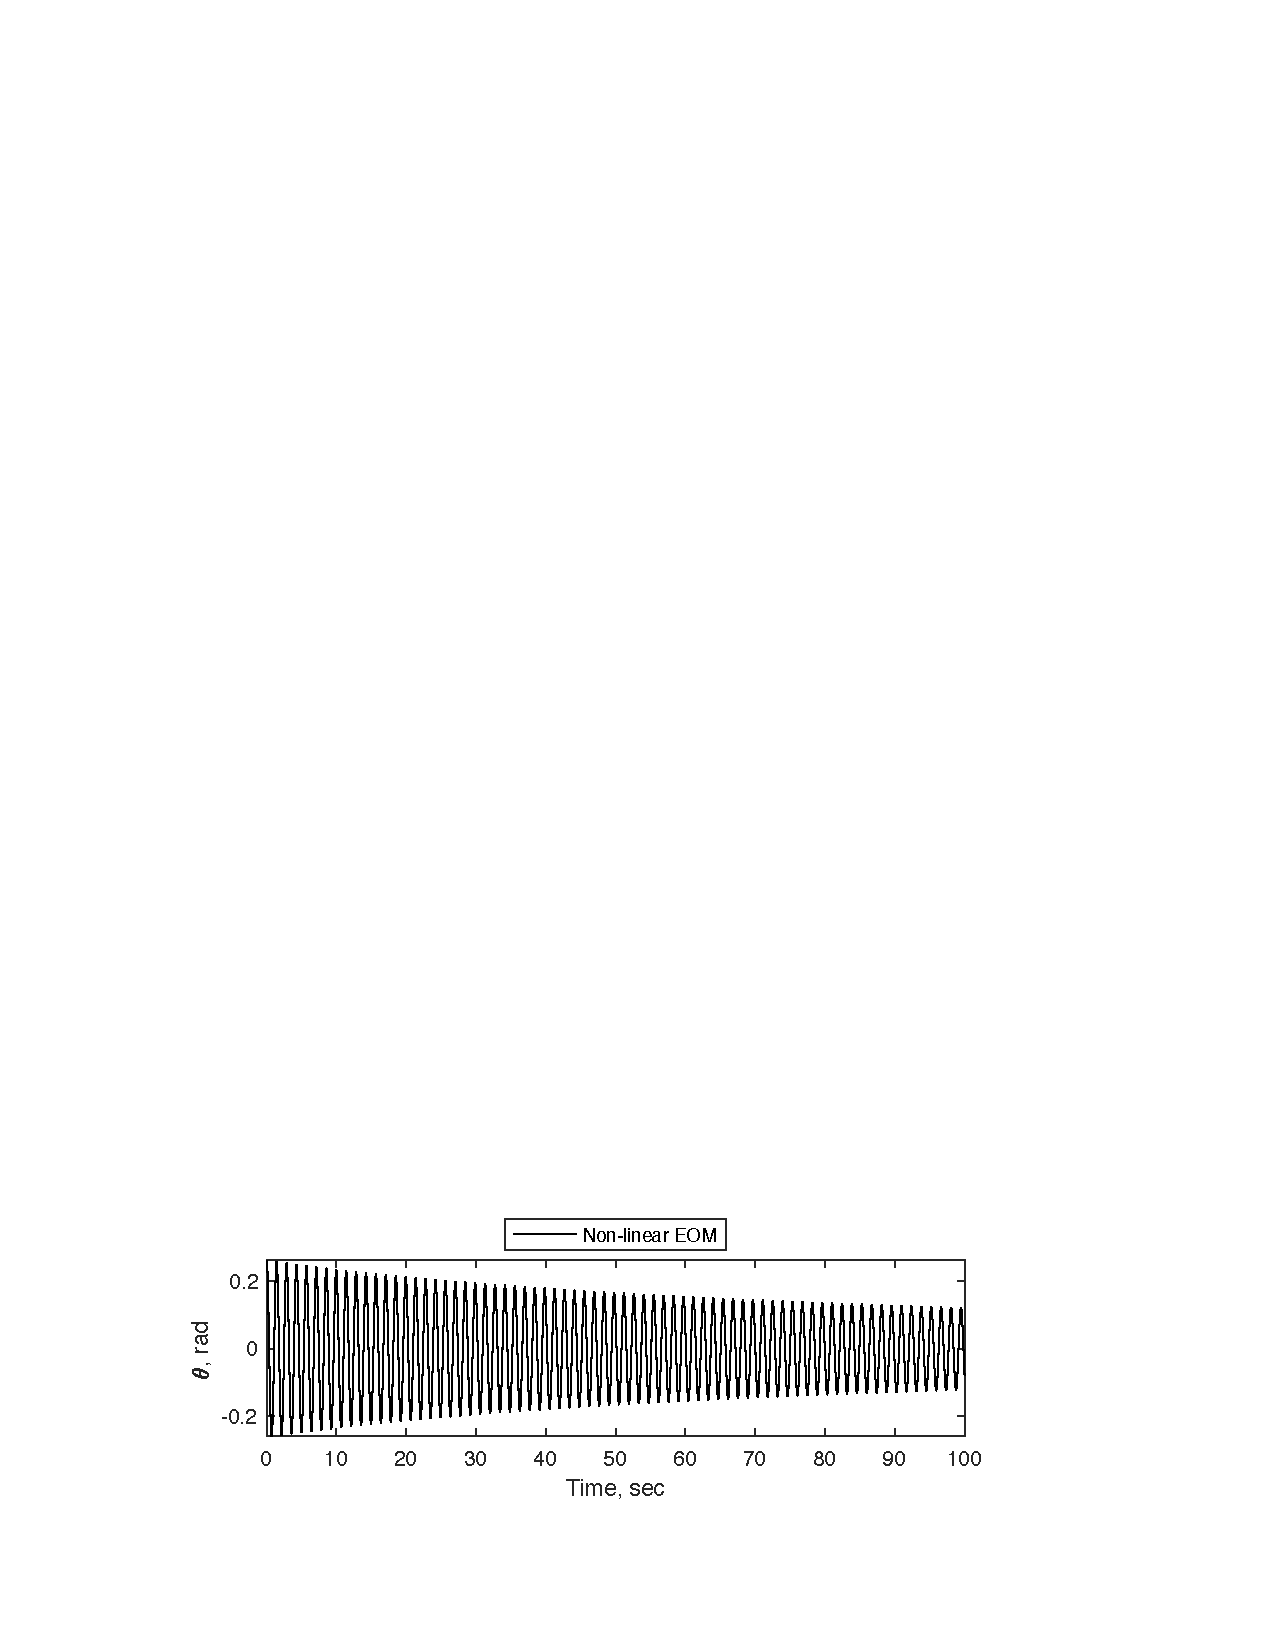
\includegraphics[center]{thetadrag}
  \caption{$\theta$ vs Time with Drag}
  \label{fig:thetadrag}
\end{figure}
We can see the amplitude of the pendulum oscillations decreasing over time.
We then determine the second order differential equation that correctly models
the system with drag to be.
$$\ddot{\theta}+2\zeta\omega_n\dot{\theta}+\omega_n^2\theta=0$$
Solving the second order differential equation we produce,
\begin{equation} \label{eq:thetat}
\theta(t)=e^{-\zeta\omega_nt}(A\cos(\omega_dt)+B\sin(\omega_dt))
\end{equation}
When $\theta(0)$ and $\dot{\theta}(0)$ are evaluated they yield the equation
$$-\zeta\omega_nB+\omega_dA=0 \quad\therefore\quad A=\frac{\zeta\omega_nB}{\omega_d}$$
Plugging A and B into (\ref{eq:thetat}), the equation can be rewritten as
\begin{equation} \label{eq:thetat_verbose}
\theta(t)=\frac{\pi}{12}e^{-\zeta\omega_nt}\left(\frac{\zeta\omega_n}{\omega_d}\sin(\omega_dt)+\cos(\omega_dt)\right)
\end{equation}
\newpage
By taking the average time between the peaks based on Figure (\ref{fig:thetadrag}) we find $\omega_n=4.4211098$\\
Simplifying (Eq. \ref{eq:thetat_verbose}) we can solve for $\omega_d$
$$\omega_d = \omega_n\sqrt{1-\zeta^2} = 4.4211015$$
$\omega_d$ and $\omega_n$ are extremely close to eachother but not exactly equal.\\
This makes sense when we solve for $\zeta$ by rewriting (Eq. \ref{eq:thetat_verbose})
$$\zeta = \sqrt{\frac{\ln^2(\frac{\theta(t_p)}{\theta_o})}{\ln^2(\frac{\theta(t_p)}{\theta_o})+(2\pi N)^2}} = 0.001947$$
\\We then compare the plots of $\theta$ vs. Time from (Eq. \ref{eq:thetat_verbose}) and our EOM.\\
\begin{figure}[ht]
  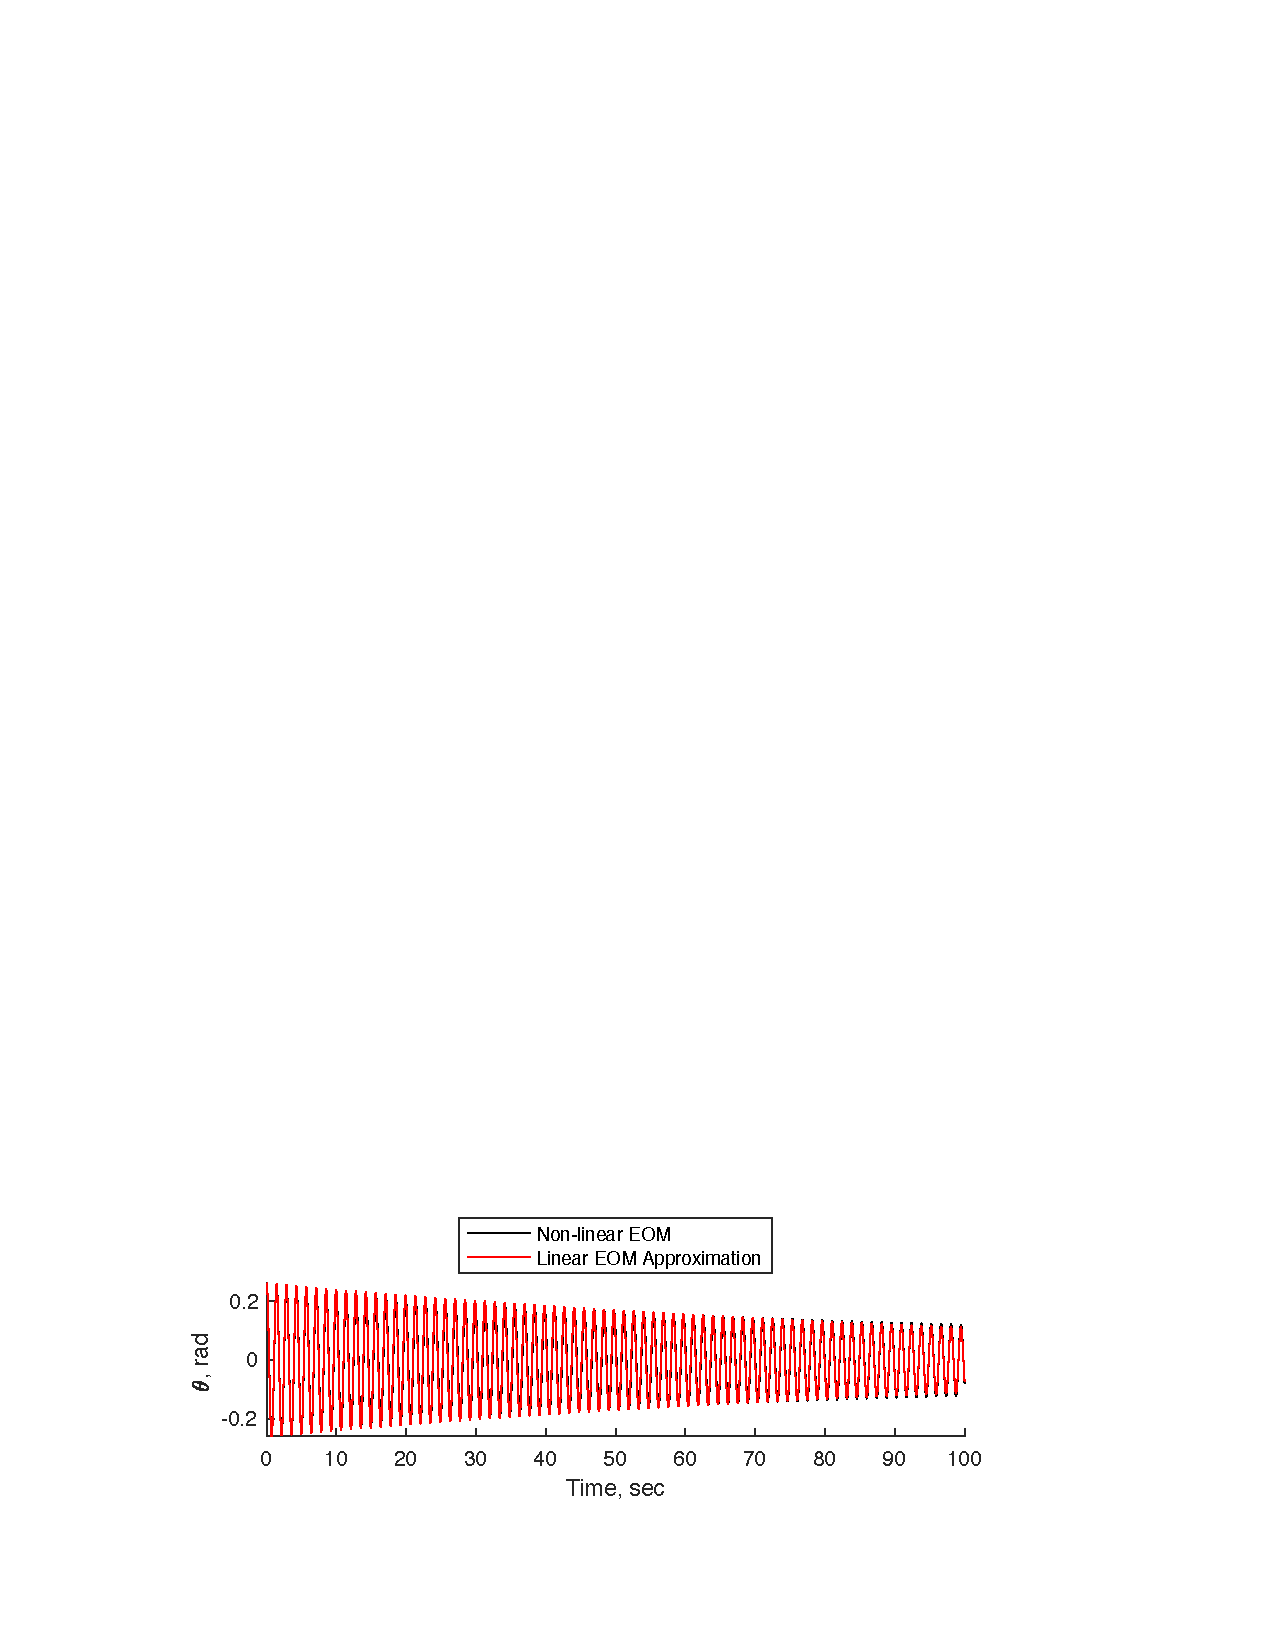
\includegraphics[center]{compare}
  \caption{$\theta$ vs Time with Drag, Non-linear vs. Linear EOM}
\end{figure}
Examining the plot more closely we can see that the Linear EOM Approximation is very close to the plot generated by the non-linear EOM. Plotting the last 5 seconds produces Figure (\ref{fig:timewithdrag}).
\begin{figure}[ht]
  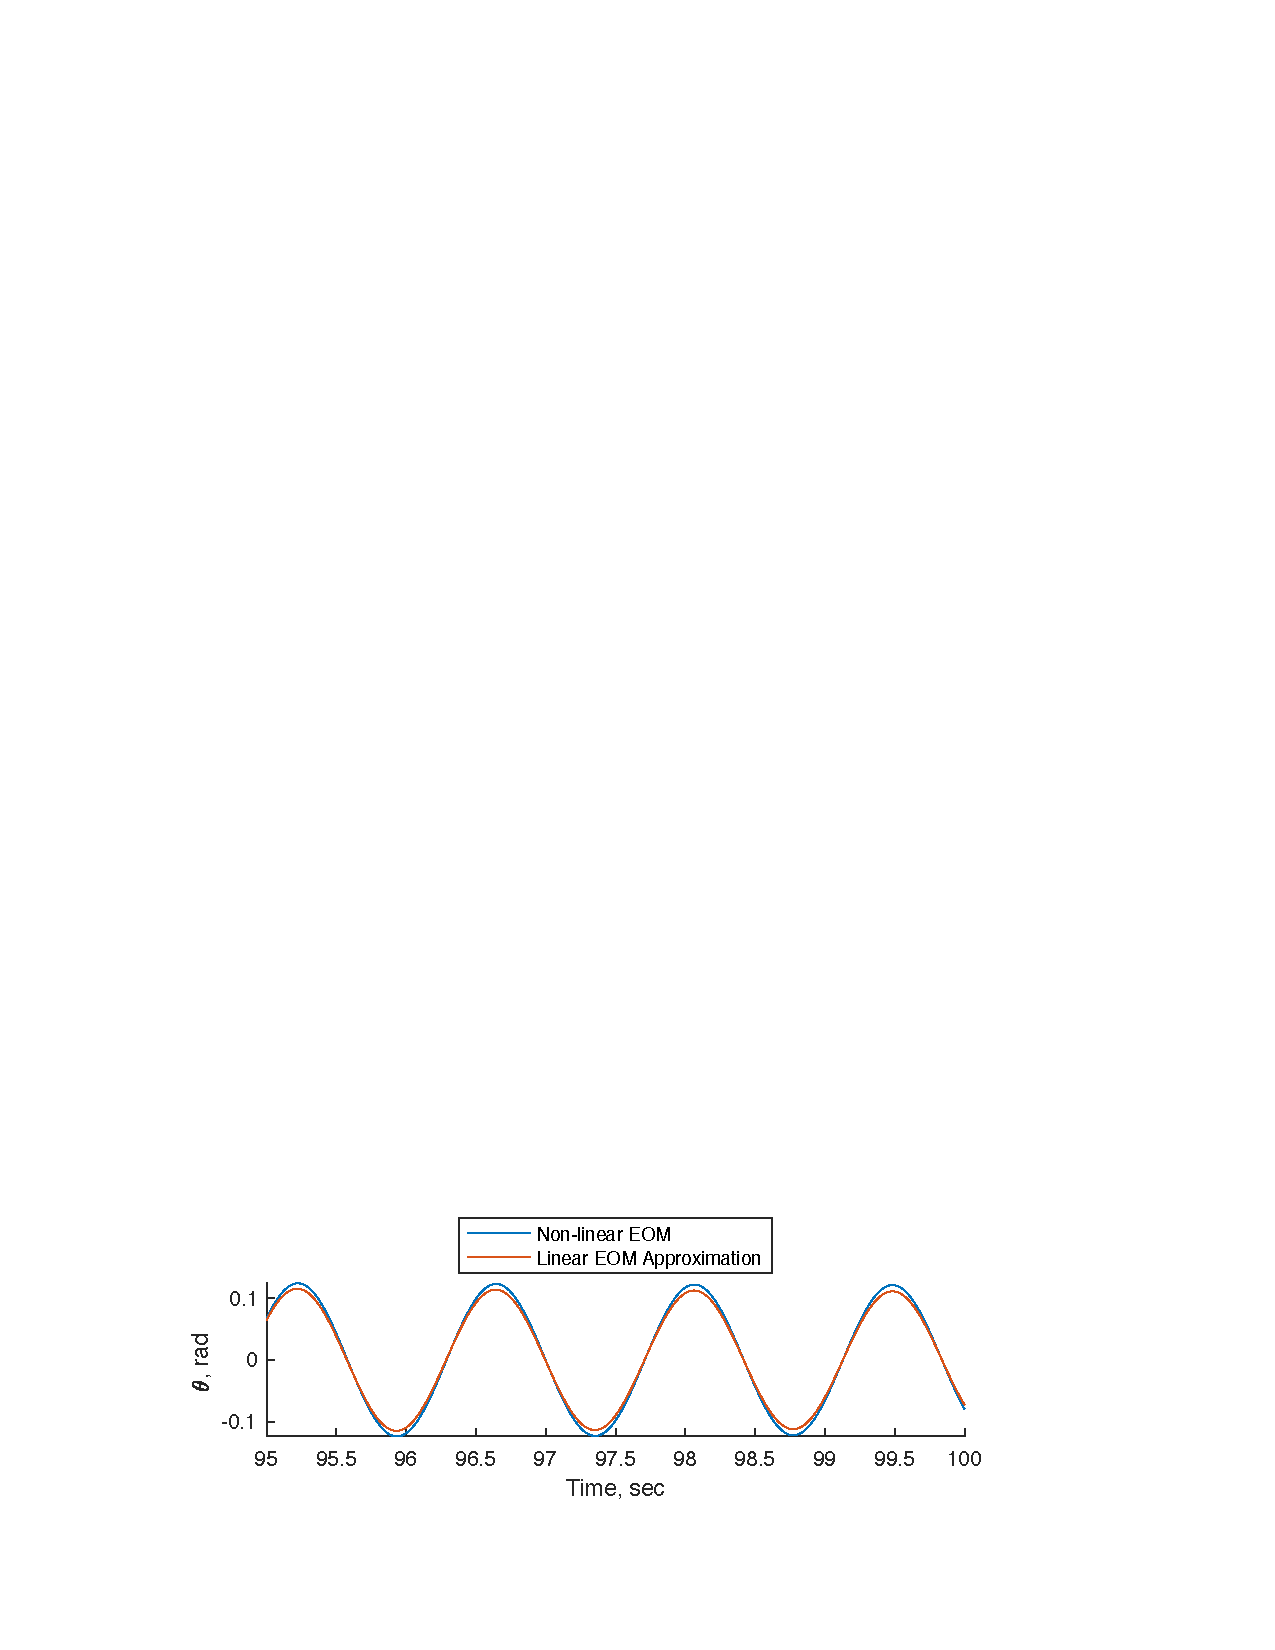
\includegraphics[center]{compareclose}
  \caption{$\theta$ vs Time with Drag, Non-linear vs. Linear EOM Magnification}
  \label{fig:timewithdrag}
\end{figure}
\newpage
% ---------------------------------------------------------------------------- %
\section{Does it Make Sense?}
% ---------------------------------------------------------------------------- %
\subsection{Units}
EOM without drag (from (\ref{eq:pen})):
$$
\ddot{\theta} = -\frac{g}{L}\sin(\theta) \quad = \quad
\frac{\frac{\cancel{m}}{s^2}}{\cancel{m}}\cdot rad = \frac{rad}{s^2}
$$
Similarly, with the small angle approximation,
$$
\ddot{\theta} = -\frac{g}{L}(\theta) \quad = \quad
\frac{\frac{\cancel{m}}{s^2}}{\cancel{m}}\cdot rad = \frac{rad}{s^2}
$$
Looking at the EOM with drag (from (\ref{eq:drageom})), since the final units still need to come out to $\sfrac{rad}{s^2}$, the drag term must have the units kg $\cdot$ m in order to cancel out: \\
$$
\ddot{\theta} = -\frac{g}{L}\sin(\theta) - \frac{1.65 \cdot 10^{-3}\dot{\theta}|\dot{\theta}|}{mL} \quad = \quad
\frac{\frac{\cancel{m}}{s^2}}{\cancel{m}} \cdot rad - \frac{\cancel{kg} \cdot \cancel{m}\cdot \sfrac{rad}{s^2}}{\cancel{kg}\cdot\cancel{m}}
=
\frac{rad}{s^2}
$$
~\\
Checking with the MATLAB symbolic units tool (from Section \ref{appendix:numerical}): \\
~\\
\begin{lstlisting}[frame=lines,style=Matlab-editor]
% Checking EOM Units
u = symunit;
m = m*u.kg;
g = g*u.m/u.s^2;
l = l*u.m;
k = k*u.N/u.m;
An = An*u.N;
At = At*u.N;
Cn = Cn*u.N;
Ct = Ct*u.N;
theta = 'theta';
thetadot = 'thetadot'/u.s;
thetaddot = 'thetaddot'/u.s^2;
phi = 'phi';
phidot = 'phidot'/u.s;
phiddot = 'phiddot'/u.s^2;

eqn = subs(eqn);
unitCheck = checkUnits(eqn)
\end{lstlisting}
\color{gray} \begin{verbatim}
unitCheck = 
  struct with fields:

    Consistent: [1 1 1 1 1 1]
    Compatible: [1 1 1 1 1 1]
\end{verbatim} \color{black}

\newpage
\subsection{Magnitude}
Without Drag: \\
~\\
Looking at Figure (\ref{fig:thetatime}), the amplitude of the oscillations show no
deterioration, which is consistent for a system with no outside forces (such as drag).
As the initial angle of realease ($\theta_o$) and the period of ocsillations increase, the
natural frequency ($\omega_n$) decreases, which makes physical sense. Also, as seen in
Figure (\ref{fig:freq}), the natural frequency of the system with small initial angles
show that the small angle approximation ($\sin(\theta) \approx \theta$) is valid,
because they approach $\sqrt{\frac{g}{L}}$ which is $\omega_n$ with $\sin(\theta) \approx \theta$.

~\\
With Drag: \\
~\\
Now, looking at Figure (\ref{fig:thetadrag}), we can see that the amplitude of the
oscillations is slowly decreasing over time, showing a loss in energy due to the
drag component included the system. The natural frequency ($\omega_n$) and the damped
natural frequency ($\omega_d$) are very close in magnitude. This makes physical sense because
the damping ratio ($\zeta$) is very small, and will only affect the system in small amounts.

~\\
Signs: \\
~\\
Given the coordinate system discussed in Section (\ref{knownsandunknowns}) and the
equations of motion with and without drag, (\ref{eq:pen}) \& (\ref{eq:drageom}), \\
~\\
When $\theta_o > 0$, the initial angular acceleration ($\ddot{\theta_o}$) is negative,
or swinging towards the position with the least energy ($\theta = 0$). \\
When $\theta_o < 0$, the initial angular acceleration ($\ddot{\theta_o}$) is positive,
or swinging towards the position with the least energy ($\theta = 0$). \\
~\\
Both of these situations make physical sense.
\newpage
\section{Appendix} \label{appendix}

\subsection{Attributions}

\onehalfspacing
\begin{tabular}{ll}
Jeffrey Chen & Conceptualization, Solving Damped/Natural Frequencies\\
Thorne Wolfenbarger & Solving Damped/Natural Frequencies, Write-up\\
Trey Dufrene & Free Body/Coordinate System, Step 9, Write-up\\
Joint Effort & MATLAB Coding, Solving EOM's
\end{tabular}
\singlespacing

\subsection{Analytical Solution}
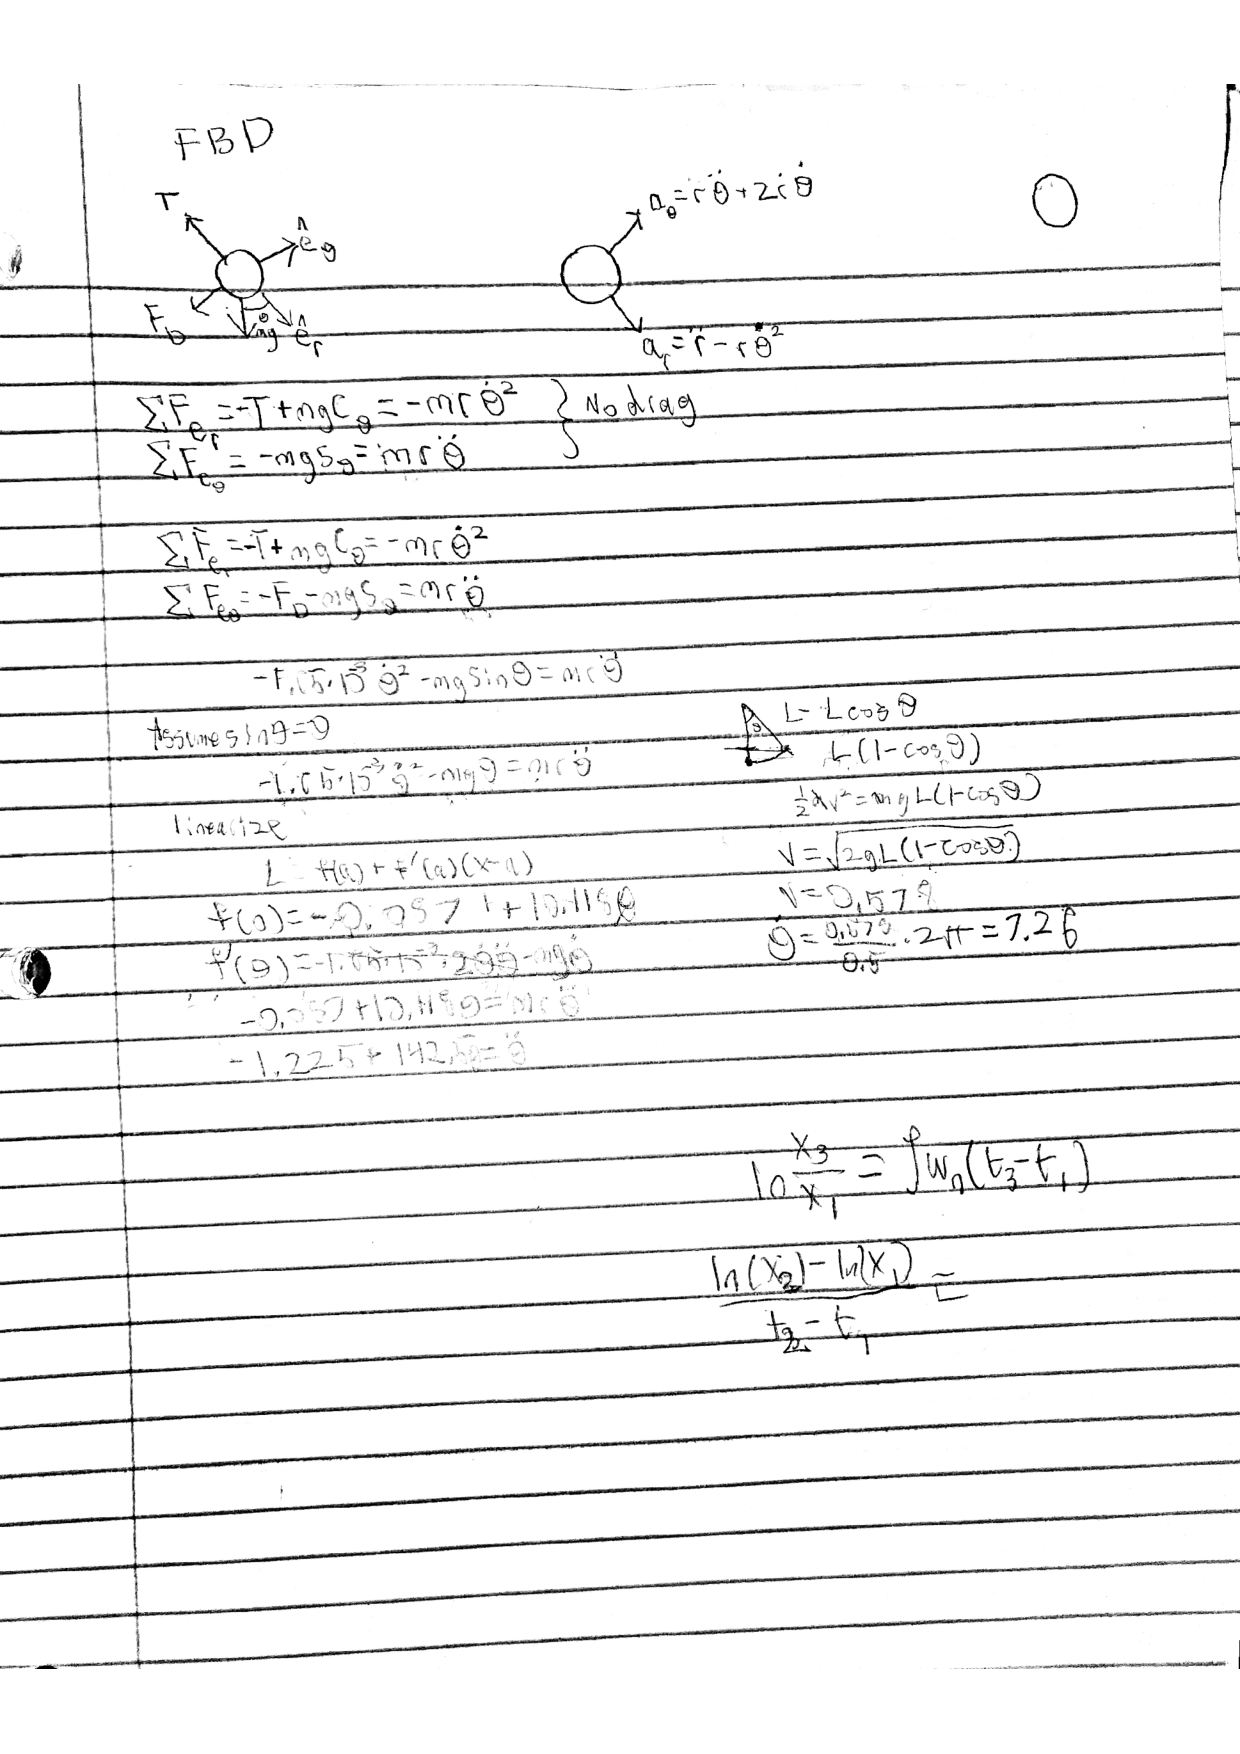
\includegraphics[frame, width=\textwidth]{analytical}
\newpage

\subsection{Numerical Solution} \label{appendix:numerical}
\subsubsection{Without Drag}
\begin{lstlisting}[frame=lines,style=Matlab-editor]
% Declaring Constants
c.g = 9.81; % ms/s^2
c.m = 0.142; % kg
c.L = .5; % m

options = odeset('Events', @event);

% Declaring Variables
syms m g L theta thetadot thetaddot T

% Our Equations of Motion (EOM)
eqn(1) = m*(L*thetadot^2) == T - m*g*cos(theta);

eqn(2) = (thetaddot) == (-m*g*sin(theta))/(m*L);

% Solve our EOM and integrate it in ode45
x = solve(eqn,[T,thetaddot]);

syms theta(t) thetadot(t)
thetaEOM = subs(x.thetaddot,{'theta','thetadot'},...
               {theta,thetadot});
eom = odeFunction([thetadot;thetaEOM],[theta;thetadot],g,L);

hold on;
% Plotting our Data for Theta Time History for System With Drag at
% different angles
nat_freq = zeros(1,6);
releaseAngle = [5,10,15,30,60,90];
for i = 1:6
    j = releaseAngle(i);
    [Time,S,TE,SE,IE] = ode45(@(t,s)eom(t,s,c.g,c.L),linspace(0,10,1001),[(j*pi/180),0],options);
    plot(Time,S(:,1),'DisplayName', ['\theta_o = ' num2str(j) '^o']);
    xlabel('Time, sec');
    ylabel('\theta, rad');
    nat_freq(i) = 2*pi / (TE(2))
end
title('\theta vs Time');
legend('show')

%Graph of natural frequencies
figure(2)
hold on
plot(releaseAngle*pi/180,nat_freq, 'DisplayName', 'Measured Natural Frequency')
line([0  90].*pi/180, [sqrt(c.g/c.L),sqrt(c.g/c.L)],'Color','red','LineStyle','--',...
    'DisplayName',['Small Angle Approximation Natural Frequency'])
xlabel('\theta_o, rad');
ylabel('\omega_n, rad/s');
xticks([5*pi/180 pi/18 pi/12 pi/6 pi/3 pi/2])
xticklabels({'5\pi/180','\pi/18','\pi/12','\pi/6','\pi/3','\pi/2'})
xtickangle(45)
grid on
legend('show')
legend('location', 'northoutside')

set(gcf, 'PaperPositionMode', 'manual');
set(gcf, 'PaperUnits', 'inches');
set(gcf, 'PaperPosition', [1 1 6 2.5]);
fig = gcf;
print('BestFitFigure','-dpdf');


% Event function
function [value isterminal direction] = event(t,s)
    value = s(2);
    isterminal(1) = false;
    direction(1) = -1;
end
\end{lstlisting}

\color{gray} \begin{verbatim}
nat_freq =
    4.4278    4.4215    4.4110    4.3543    4.1292    3.7578
\end{verbatim} \color{black}

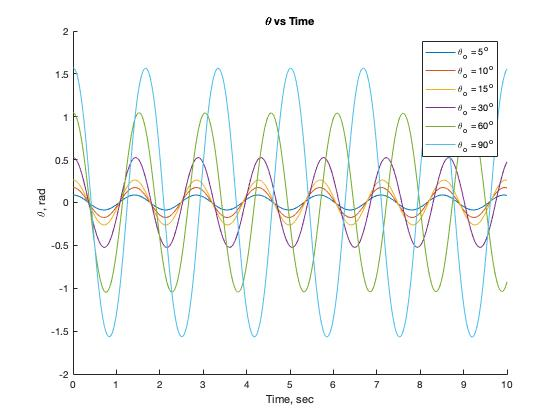
\includegraphics [width=5in,center]{Pendulum_01.jpg}

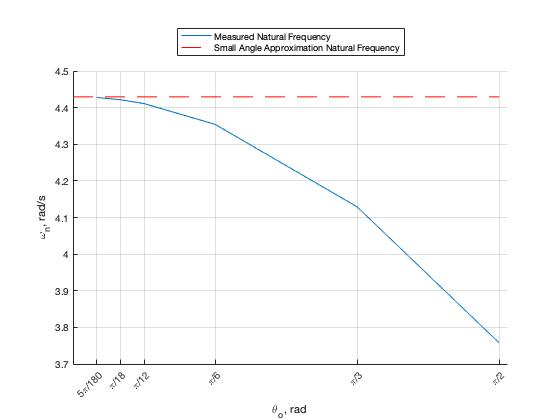
\includegraphics [width=5in,center]{Pendulum_02.jpg}

\newpage
\subsubsection{With Drag}
\begin{lstlisting}[frame=lines,style=Matlab-editor]
% Declaring Constants
c.g = 9.81; % ms/s^2
c.m = 0.142; % kg
c.L = .5; % ft

options = odeset('Events', @event);

% Declaring Variables
syms m g L theta thetadot thetaddot T
% Our Equations of Motion (EOM)
eqn(1) = m*(L*thetadot^2) == T - m*g*cos(theta);
eqn(2) = (thetaddot)*(m*L) == (-m*g*sin(theta)) - (1.65*10^-3)*thetadot*(abs(thetadot));

% Solve our EOM and integrate it in ode45
x = solve(eqn,[T,thetaddot]);

syms theta(t) thetadot(t)
thetaEOM = subs(x.thetaddot,{'theta','thetadot'},...
               {theta,thetadot});
eom = odeFunction([thetadot;thetaEOM],[theta;thetadot],g,L,m);

[Time,S,TE,SE,IE] = ode45(@(t,s)eom(t,s,c.g,c.L,c.m),linspace(0,100,10001),[(15*pi/180),0],options);

% Plotting our Data for Theta Time History for System With Drag
figure(1)
plot(Time,S(:,1),'-k')
xlabel('Time, sec')
ylabel('\theta, rad')
legend('Non-linear EOM','Linear EOM Approximation')
legend('location', 'northoutside')
legend('show')
set(gcf, 'PaperPositionMode', 'manual');
set(gcf, 'PaperUnits', 'inches');
set(gcf, 'PaperPosition', [1 1 6 2]);
fig = gcf;
print('ThetaVsTimeWithDrag','-dpdf');

%Calculating omega_d, zeta, and omega_n
mean_period_time = mean(diff(TE));
omega_d = (2*pi/mean_period_time);
decayRate = mean(log(SE(2:end,1)./(SE(1:end-1,1)))./(TE(2:end)-TE(1:end-1)));
zeta = [];
for i = 1:length(TE)
zeta(i) = ...
sqrt((log(SE(i,1)./(15*pi/180)).^2)./((log(SE(i,1)./(15*pi/180)).^2)+(2*pi*i)^2) ...
);
end
zeta = mean(zeta);
omega_n = omega_d/sqrt(1-zeta^2);
% Theta in terms of omega_d, zeta, and omega_n
theta_func = pi/12 .* exp(-zeta*omega_n.*Time) .* (zeta*omega_n/omega_d .* sin(omega_d.*Time)+cos(omega_d.*Time));
figure(2)
% Plotting Time vs theta
xlabel('Time, sec')
ylabel('\theta, rad')
hold on
plot(Time,S(:,1),'-k')
plot(Time,theta_func,'-r')
hold off
legend('Non-linear EOM','Linear EOM Approximation')
legend('location', 'northoutside')
legend('show')
set(gcf, 'PaperPositionMode', 'manual');
set(gcf, 'PaperUnits', 'inches');
set(gcf, 'PaperPosition', [1 1 6 2]);
fig = gcf;
print('CompareLinearAndNonLinear','-dpdf');

figure(3)
% Plotting Time vs theta on a short duration
xlabel('Time, sec')
ylabel('\theta, rad')
hold on
plot(Time(9500:end),S(9500:end,1))
plot(Time(9500:end),theta_func(9500:end))
xlim([95 100])
hold off
legend('Non-linear EOM','Linear EOM Approximation')
legend('location', 'northoutside')
legend('show')

set(gcf, 'PaperPositionMode', 'manual');
set(gcf, 'PaperUnits', 'inches');
set(gcf, 'PaperPosition', [1 1 6 2]);
fig = gcf;
print('CompareLinearAndNonLinearLast5Seconds','-dpdf');

% Event function
function [value isterminal direction] = event(t,s)
    % value is a function that is zero at the event
    % isterminal is 1 if you desire to terminate integration at the event
    %               0 if you desire to continue integration
    % direction defines the slope of the function value at the event
    %      1 for positive slope, -1 for negative slope, 0 for either
    % event 1: max position
    value = s(2);
    isterminal = false;
    direction = -1;
end
\end{lstlisting}

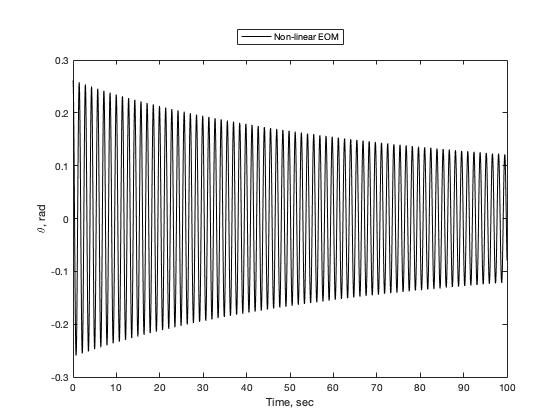
\includegraphics [width=5in,center]{PendulumThorne_01.jpg}

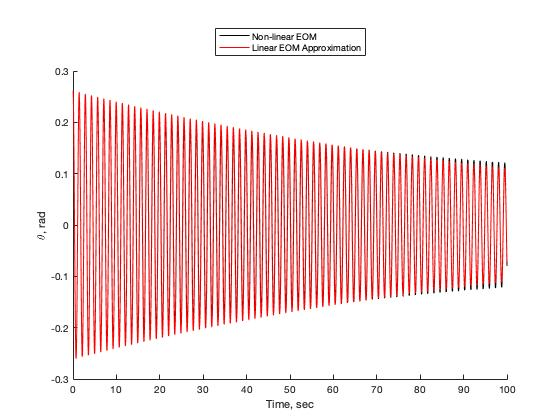
\includegraphics [width=5in,center]{PendulumThorne_02.jpg}

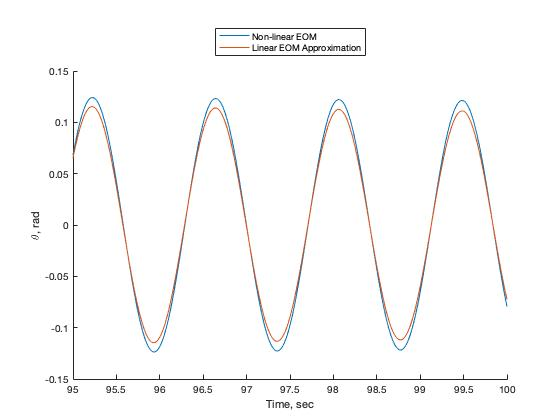
\includegraphics [width=5in,center]{PendulumThorne_03.jpg}


\end{flushleft}
\end{document}
